\documentclass[shortabstract, inz, english]{iithesis}
\usepackage[english]{babel}
\usepackage[utf8]{inputenc}
\usepackage[T1]{fontenc}
\usepackage{subcaption}
\usepackage{float}
\usepackage{amsmath,amssymb}
\usepackage{mathabx}
\usepackage{adjustbox}
\usepackage[utf8]{inputenc}
\usepackage{hyperref}
%\usepackage[backend=biber,style=numeric,sorting=none]{biblatex}
\usepackage{csquotes}
\usepackage{graphicx}
\usepackage{caption}

\DeclareMathOperator{\mnistM}{MNIST-MNIST-M}
\DeclareMathOperator{\svhnM}{SVHN-MNIST}
\DeclareMathOperator{\QCM}{MNIST}
\DeclareMathOperator{\QCMM}{MNIST-M}

\captionsetup[table]{skip=3pt}
\captionsetup[figure]{skip=5pt}

\newcommand{\mnist}{$\overline{\mnistM}$ }
\newcommand{\svhn}{$\overline{\svhnM}$ }
\newcommand{\CM}{$C_{\QCM}$}
\newcommand{\CMM}{$C_{\QCMM}$}

\englishtitle{Experiments with unsupervised domain adaptation using the gradient reversal layer}
\polishtitle{Eksperymenty z nienadzorowaną adaptacją dziedzinową przy użyciu gradient reversal layer}
\author{Wojciech Pratkowiecki}
\advisor{dr Jan Chorowski}
\date{15 lutego 2019} 


\englishabstract{
The amount of data that is still unlabeled has been growing over recent years. With domain adaptation methods it is possible to get a model that classifies well these samples, if only a related and labeled set is available. While trying to get better and better classification results, many diverse and complex approaches were invented. This paper describes analysis and experiments aimed at understanding the problem of domain adaptation and coping with it using the \textit{gradient reversal layer} and its modifications.
}

\polishabstract{
Ilość danych, które wciąż nie zostały opisane, znacznie wzrosła na przestrzeni ostatnich lat. Dzięki adaptacji dziedzinowej możemy otrzymać model, który poprawnie klasyfikuje takie dane, jeżeli tylko posiadamy zbiór powiązanych, opisanych przykładów. Aby uzyskać jak najlepsze wyniki klasyfikacji, wymyślono wiele różnorodnych i skomplikowanych metod. Ta praca opisuje analizy oraz eksperymenty, których celem jest zrozumienie samego problemu adaptacji dziedzinowej, jak i radzenia sobie z nią przy użyciu \textit{gradient reversal layer} oraz jego modyfikacji. 
}

\begin{document}

\chapter{Introduction}
Neural networks have found many applications in recent years due to their ability of learning some complex data dependencies. Top performance in various tasks have resulted in increased popularity of not only neural networks and deep learning but also of other machine learning (ML) methods. Different architectures designed for different tasks were invented. One of them is convolutional neural network (CNN) introduced by Yann LeCun \cite{cnn}, which caused huge improvement in the image classification field. However, obtaining top-performing models often requires a long training, with huge amount of labeled data. Such a complicated procedure yields a desired model, but it would not reach comparable results on different, even strongly related dataset. Moreover, if we  have small amount of labeled samples, we need to find an alternative way to train the network. At this point domain adaptation is an attractive option.
\par
Domain adaptation (DA) is a process of learning a distribution of samples from source domain and obtain a model that performs well on other, but related, target domain. For instance, if we have a huge (e.g. synthetic), labeled set of road signs images and a video from a ride through a city, we could get an effective model that classifies well all the signs from the video frames, if we train it properly with the labeled dataset. One of domain adaptation techniques is the gradient reversal layer (GRL) proposed by Yaroslav Ganin and Victor Lempitsky \cite{pmlr-v37-ganin15}. GRL is a simple, but effective, architectural trick, applied during backpropagation, designed especially for domain adaptation task. This thesis is a collection of research on the gradient reversal layer and its adjustments, with some new approaches and modifications that may not only improve its accuracy, but also help to get a detailed understanding of domain adaptation problem and the GRL behaviour.

\chapter{Background knowledge}
\section{Artificial neural network}

Artificial neural network (ANN) is a machine learning technique inspired by the neural connections in human brain. While training the model we use a pre-defined architecture and a loss function. The architecture describes the transformation of the input data made by our model, its complexity and interpretation of the output. Each network contains neurons that are stacked in layers. Neurons are nothing but a weighted sum characterized by the neuron's weights and bias. A layer is built with many neurons and followed by non-linear activation function. Each layer transforms its input vector into an output vector. The first layer of the network is called the input layer, the last one is the output layer, while all the intermediate layers are called hidden layers. Figure~\ref{fig:ANN} presents a sample ANN. The loss function is a way to measure and optimize the performance of the model, it is commonly the magnitude of its imprecision.
\par
Successful learning process requires many examples of the problem we want the network to solve. At the beginning, we usually set the model's parameters (mostly denoted as $\Theta$) to random values. The model transforms some of the input examples and we compute the loss function based on the output. As we want the model to perform as well as possible, our goal is to minimize the loss function. Therefore we use the backpropagation method - for each input sample we compute its gradient. The values of those gradients tell us, how should we tune model's parameters $\Theta$ to find the minimum of loss function. Therefore, we slightly change values of $\Theta$ in the direction of gradient, which should recall in a better performance of the model on the next examples. We repeat this process many times, improving our network during the whole learning process. 
\par
This iterative training approach is a simplified description of stochastic gradient descent (SGD) - one of the most popular and effective ANN optimization method. As our model may be defined by millions of parameters, computational cost of thousands of training iterations is a huge drawback of neural networks. However, great growth of computer's computation power with GPU acceleration let us find solutions for some really complex problems within a decent time.  Therefore neural networks are nowadays widely used for many tasks. One of them is image classification - finding for a given input image the most likely label from a fixed label set.

\section{Convolutional neural networks}
Applying neural networks to image processing became very popular. To keep reaching better results in tasks, like image classification, some new inventions were needed. The breakthrough came with convolutional neural networks (CNN). CNN, just like classical neural network, is built with neurons stacked in layers. First layers of CNN are convolution layers. Each of them is a set of learnable, small size (like 5$\times$5) filters followed by activation function. Each filter processes an input image step by step and produces a transformed, usually smaller, one. Therefore, after each layer we get a new set of images obtained from all pictures from previous layer. A big advantage of this approach is a much smaller number of learnable parameters - if the input image has size 1000 $\times$ 1000 it would require 1000000 parameters for a single neuron in a fully connected layer, while convolution layer processes it with its filter, that has 25 parameters, if the size of the filter is 5$\times$5.  After a convolution layer we usually use pooling - we divide the picture into cells (e.g. of size 2$\times$2) and we replace the whole cell with its maximum value (in case of the maximum pooling). This operation reduces the size of the image internal representation, and force the network to focus on important patterns. Figure~\ref{fig:CNN} presents an example of CNN architecture.
\par
The convolutional part of the model learns high-level features or descriptors of locations in the input image. Moreover it makes the network invariant for small translation of object over the image. Convolutional layers produce a vector representation of the input image. It is then fed into classical, fully-connected layers that return the model's output. If our task is image classification the output is a vector of classes probabilities typically.
\par
CNNs caused huge improvements in both accuracy and speed of image classification. Nowadays top-performing architectures in many image processing problems are built with convolutions. Convolutional layers also found application in some non-picture field like some natural language processing tasks or speech generation. 

\begin{figure}[htb]%
    \centering
    \includegraphics[width=\linewidth]{ANN.jpeg}%
    \caption{Example of neural network architecture. Picture from Stanford course website \cite{stanford}}%
    \label{fig:ANN}%
\end{figure}
\begin{figure}[htb]%
    \centering
    \includegraphics[width=\linewidth]{CNN.png}%
    \caption{Example of convolutional neural network architecture. Picture from \cite{cnn_im}}%
    \label{fig:CNN}%
\end{figure}

\section{Digit classification with CNN}
MNIST dataset \cite{mnist} is a collection of black and white photos of handwritten digits. Every picture's resolution is 28$\times$28 pixels, each one is an integer in the range $[0,255]$, that describes the brightness of the pixel. All the samples are provided with ground truth labels. Classification of digit images is therefore a task of processing the input image that dimensionality is 28$\times$28, and assigning probabilities for each of 0-9 digits. The model prediction is the digit with highest probability. Even very ordinary convolutional architecture reaches over 99\% accuracy on this dataset. A bit more challenging modification of MNIST is the MNIST-M set \cite{mnist-m}, obtained by blending example from MNIST with some color photos from BSDS500. There is probably no difference in difficulty of classification MNIST and MNIST-M digits for human, but from neural network point of view, the colorful set is much more complex. Nevertheless, obtaining top-performing model is relatively easy.
\par
There are a lot of similar digit recognition datasets, with many that are much more complex than MNIST and its modifications. The Street View House Number (SVHN) is a good example of such collection. SVHN samples are obtained from Google Street View photos, therefore they are colorful, with diverse backgrounds, pictures are often blurry and a single image may present few digits, while its label is the one in the centre of the photo. Due to all those properties of SVHN, model that classifies well its samples must be complex and longer trained. 
\par
Even though digit classification seems not to be the most important and entertaining problem that CNN may solve, it is still one of the most popular field of measuring a model's performance and yields experimental results with quick turn-around time. Figure~\ref{fig:digits} presents some examples from mentioned datasets - MNIST, MNIST-M and SVHN.

\begin{figure}%
    \centering
    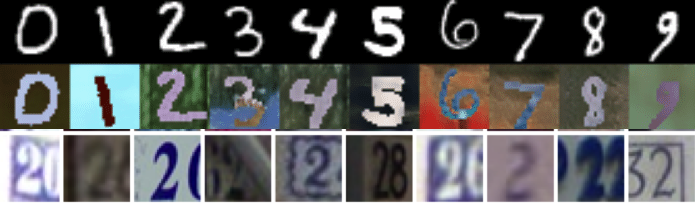
\includegraphics[width=\linewidth]{digits.png}%
    \caption{Samples from MNIST, MNIST-M and SVHN digit images datasets, best viewed in color}
    \label{fig:digits}%
\end{figure}

\section{Domain adaptation}
Let's suppose that we have a novel, large set of digit images, for instance photos of the back of each European footballer's jersey, preprocessed in a way, that every image contains one digit - figure~\ref{fig:football} presents some possible samples. Our goal is to obtain a model that classifies digits from football kits. Unfortunately we don't have any labels for these pictures, so we are unable to go a straightforward way and train a CNN adjusted to the image set, as we cannot determinate if the model's prediction is right. In this kind of situation domain adaptation is a solution.
\par
Domain adaptation is a specific training process, when we teach a model with examples from a source domain, but our goal is to make it perform well on different, but related, target domain. Over recent years many architectures have been proposed to reach as high target domain accuracy as possible. DA is needed when samples from target distribution are unlabeled (unsupervised domain adaptation) or we have just few labeled examples (semi-supervised domain adaptation). A model should find a mapping between domains, which would allow source domain classifier perform well on test (target domain) examples.
\par
In our case of football jerseys, when the set is unlabeled at all, we have an unsupervised DA problem. Target domain is the distribution of jersey's photos. Now we should try to obtain a model learned with labeled examples from other dataset, like SVHN, and apply some architectural solution that would let the model classify well digits from football kits. Dozens of such tricks have been proposed in recent years. One of them is gradient reversal layer.

\begin{figure}%
    \centering
    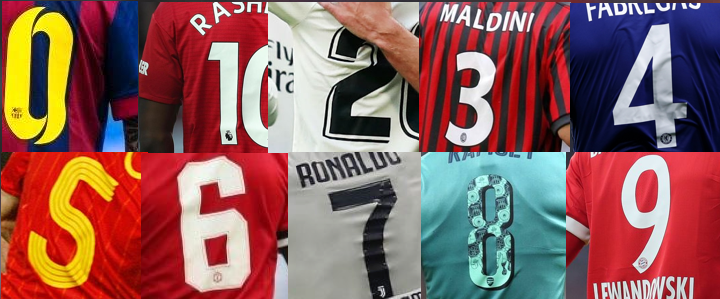
\includegraphics[width=\linewidth]{football.png}%
    \caption{Football jersey dataset}
    \label{fig:football}%
\end{figure}


\section{Domain adaptation using GRL}
Gradient reversal layer was introduced by Yaroslav Ganin and Victor Lempitsky in the paper titled "Unsupervised Domain Adaptation by Backpropagation" in 2015 \cite{pmlr-v37-ganin15}. The authors describe domain adaptation as a problem of finding common mapping for source and target distribution, that would transform samples to some kind of representation, that does not contain any information about the domain of mapped input. Therefore, the classifier basing on a transformed sample, would have similar accuracy for both distributions. In perfect scenario the mapping does not influence the label predictor's accuracy, but is so invariant w.r.t. domain shift, that we cannot obtain a well performing distribution classifier. 

\par
To obtain the desired representation, the model is divided into three parts - a \textit{feature extractor}, that is denoted as $G_{f}$ with its parameters $\Theta_{f}$. $G_{f}$ maps the input to a $D$-dimensional vector $f \in \mathbb{R}^{D}$. This representation is then used by two other components of the model - a \textit{class predictor} $G_{y}$ with parameters $\Theta_{y}$, that classifies the feature vector, and a \textit{domain predictor} $G_{d}$ with its parameters denoted as $\Theta_{d}$, which task is to predict the domain of the vector $f$.
\par
All these three components are independent neural networks that construct our architecture. While training the model we aim to force $G_{f}$ to yield domain invariant feature vectors $f$. Therefore, GRL is placed between the feature extractor $G_{f}$ and the domain predictor $G_{d}$. Its task is to change the $G_{f}$ to \textbf{maximize} the loss of the domain predictor, while $G_{d}$ itself tries to minimize its own loss function to make better predictions. If the domain predictor, that wants to does its best, is unable to to predict from which domain a sample has come from, then $f$ is getting more domain invariant. In perfect scenario GRL has such an impact on $\Theta_{f}$, that $G_{d}$ has the same accuracy as a random model. Concurrently $G_{y}$ tries to predict the class of each sample and we try to minimize its loss function. Class predictor's gradient is used to tune $\Theta_{y}$ and then passed to the feature extractor. Therefore the feature extractor parameters $\Theta_{f}$ are tuned to minimize the loss of $G_{y}$ and maximize the loss of $G_{d}$. Figure~\ref{fig:GRLarch} presents the described architecture.

\begin{figure}%
    \centering
    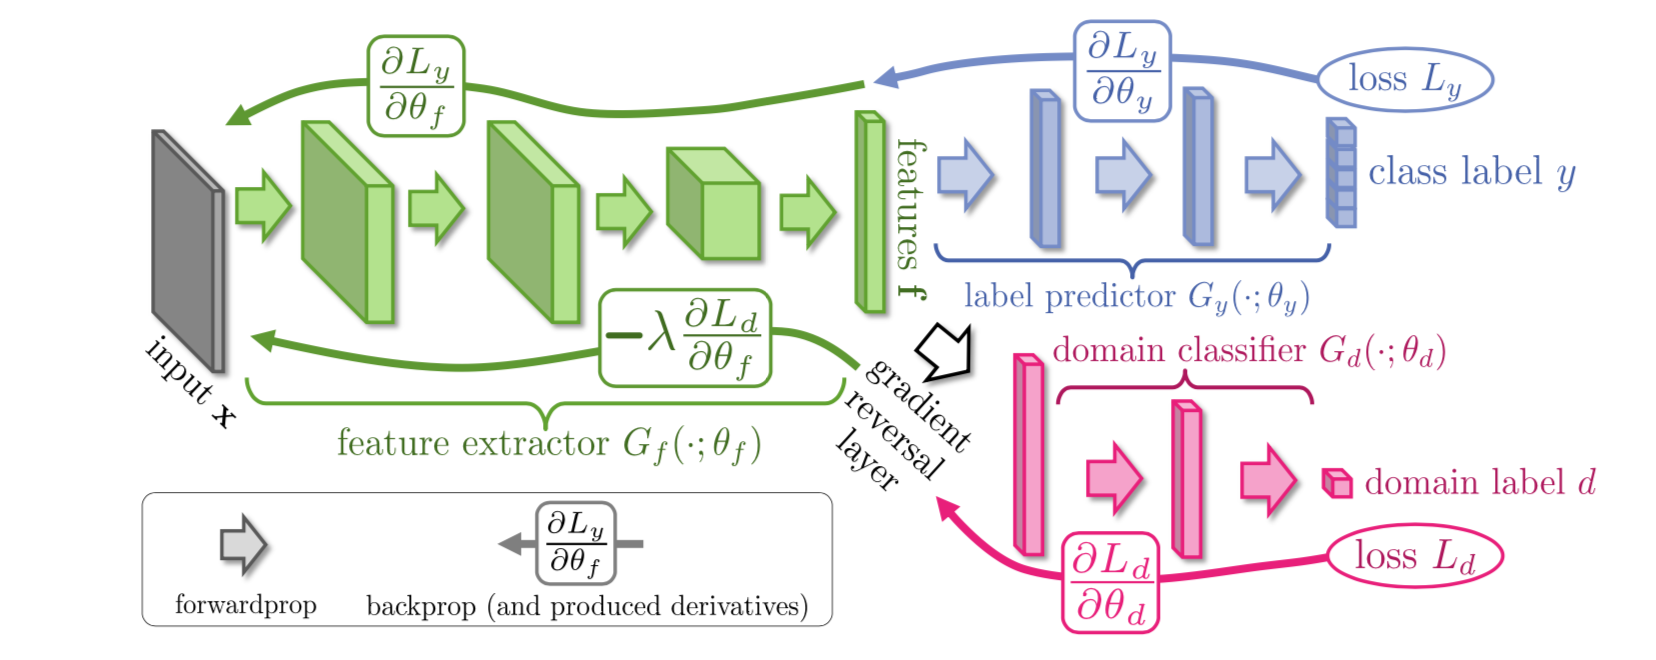
\includegraphics[width=\linewidth]{GRLarch.png}%
    \caption{Architecture with GRL in $G_{d}$ proposed by Ganin and Lempitsky - green part is a \textit{feature extractor} $G_{f}$ that transforms input sample $x$ to feature vector $f$. Afterwards it is classified by \textit{label predictor} $G_{y}$ (blue) and \textit{domain predictor} $G_{d}$ (pink). Picture from the author's paper \cite{pmlr-v37-ganin15}.}
    \label{fig:GRLarch}%
\end{figure}
\par
As the basic task of our model is to classify the digits, the parameters are tuned to make label predictor as accurate as possible. Therefore, we tune parameters $\Theta_{y}$ and $\Theta_{f}$ to minimize the loss of class predictor $L_{y}( G_y( G_{f}( x )))$. The domain predictor $G_{d}$ is tuning its parameters $\Theta_{d}$ to minimize its own loss $L_{d}( G_d( G_{f}( x )))$, but the feature extractor, as previously mentioned, tries to remove the distribution information by tuning its parameters $\Theta_{f}$ to maximize the $L_{d}$ value. Then, to find the proper parameters we perform the optimization updates:
\begin{itemize}
    \item $\Theta_{y}$ w.r.t. the direction of $-\frac{\partial L_{y}}{\partial \Theta_{y}}$ and $\Theta_{f}$ w.r.t. the direction of $-\frac{\partial L_{y}}{\partial \Theta_{f}}$
    \item $\Theta_{d}$ w.r.t. the direction of $-\frac{\partial L_{d}}{\partial \Theta_{d}}$
    \item $\Theta_{f}$ w.r.t. the direction of $\frac{\partial L_{d}}{\partial \Theta_{f}}$ (no $-$, we maximize the $L_{d}$)
\end{itemize}
\par
To perform these optimization steps we use the gradient reversal layer, as it enables us to execute this kind of updates.
Gradient reversal layer itself is a simple trick used during one forward and backward pass through the network. It is a trival layer in the network's architecture, that leaves the input unchanged during forward propagation, but multiplies the gradient by negative scalar $\lambda$ during backpropagation. We place it at the beginning of the domain predictor $G_{d}$. Therefore, the value of the gradient passed to the feature extractor is $-\lambda \frac{\partial L_{d}}{\partial \Theta_{f}}$. The $\lambda$ coefficient grows non-linearly for 0 to 1 over the training, as we want the feature extractor to focus on good representation for class predictor firstly and making the vector $f$ domain-invariant when $G_{y}$ performs well already. The optimization may be implemented then as a stochastic gradient descent update with loss $L_{y} + \lambda \cdot L_{d}$. 
\par
GRL is therefore a simple modification of model's architecture. Implementing it with some machine learning framework requires a little effort. If a model with GRL were creating absolutely domain-invariant representation of data the accuracy for test sets from source and target domain should be almost equal, as the only features left after $G_{f}$ transformation would be associated with the sample's class. During tests we don't use domain predictor, our final model is build with feature extractor and class predictor, $G_{d}$ is used only to tune parameters of the network during the training.



\section{Conceptors}
Domain adaptation is a very complex problem, therefore understanding it could be crucial to find some satisfying solutions. As previously mentioned the representation of input sample $x$ after mapping by feature extractor $G_{f}$ is a feature vector $f = G_{f}(x ; \Theta_{f}) \in \mathbb{R}^{D}$. It may be also considered as a point in $\mathbb{R}^{D}$. All the samples from source domain $S$ and target domain $T$ form a point clouds in $\mathbb{R}^{D}$ space that can be denoted as $F_{S}$ and $F_{T}$ respectively:
\begin{align*}
    F_{S} &= \{ G_{f}(x_{s} ; \Theta_{f}) : x_{s} \in S  \} \\
    F_{T} &= \{ G_{f}(x_{t} ; \Theta_{f}) : x_{t} \in T  \}
\end{align*}
\par
If the transformed samples from both domain are considered as points, the feature extractor should find a mapping, that produces as similar point clouds for distributions as possible. Then, the domain classifier could not predict well, if point from $\mathbb{R}^{D}$ with given coordinates belongs to either point cloud $F_{S}$ or $F_{T}$. Obtaining such representation would be a half way to success, as perfect mapping should also place the samples from a single class in the same region for both domains. The label predictor $G_{y}$ would then have to just find a division of the space into the regions for all classes.
\par
It is not a simple task to find a description of points cloud in $\mathbb{R}^{D}$ that would be understandable for a human, if the dimension $D$ is large. Nevertheless, it is possible to approximate these points somehow. One approach is to find an ellipsoid in $\mathbb{R}^{D}$ that captures the majority of the points. This idea was used by Herbert Jaeger to introduce the concpetors \cite{conc}. Such ellipsoid is then used to transform a new point into the cloud of known points. The conceptor is defined as a matrix $C$ that determines an ellipsoid that approximates a given point cloud and is then normalized, so it lies inside the unit sphere. Figure~\ref{fig:conceptor_intro} presents a simple visualization of this idea.
\begin{figure}%
    \centering
    \includegraphics[width=\linewidth]{c_example.png}%
    \caption{Point clouds (black) and conceptors approximating them. Best viewed in color. Picture from "Conceptors: an easy introduction" by Herbert Jaeger \cite{conc_int}. }
    \label{fig:conceptor_intro}%
\end{figure}
Singular vectors of matrix $C$ are the principal axes of the described ellipsoid, while singular values of $C$ are their lengths. The conceptor matrix $C$ is obtained with correlation matrix $R = \mathbb{E}_{x}[xx^{T}] \in \mathbb{R}^{N\times N}$ of samples $x \in \mathbb{R}^{N}$ and the aperture parameter $\alpha$, as:
\begin{equation*}
    C = R(R + \alpha^{-2} I)^{-1}
\end{equation*}
\par
The conceptors can be used to move a point inside the ellipsoid. The transformation of given point $x$ into the conceptor is made by multiplying it by the matrix $C$. If $x$ lies inside the ellipsoid that is described by the conceptor, the multiplication should act like identity and remain $x$ unchanged. If $x$ is a point from the outside of the ellipsoid then $C$ should move it inside.
\par
As it is possible to represent the high dimensional point cloud with well defined solid shape given by the conceptor, the analysis of $F_{S}$ and $F_{T}$ could be done with operations on these ellipsoids. It may be a good approach to understand the domain adaptation and the influence of GRL.

\chapter{Experiments}
\section{Paper reproduction}
First stage of all the research made within this thesis was the paper reproduction. All implementations were made with PyTorch \cite{pytorch} - deep learning python framework developed by Facebook. All computations were run on Google Colab \cite{colab} notebook. 
\par
Few architectural changes in the network proposed by Ganin and Lempitsky were made, like replacing ReLU activation function with leaky-ReLU \cite{leaky_relu} and using dropout \cite{dropout} during learning. When training on SVHN dataset, much more complex architecture was needed. The feature extractor was built with 5 convolutional layers, each one using batch normalization \cite{batch_norm} and the leaky-ReLU followed by max pooling and dropout during training process. Such a complex architecture allows us to get satisfying results 10 times faster than with model proposed by Ganin and Lempitsky\footnote{During authors' research the classification error on SVHN dataset was high for first 150 training epochs. With proposed, complex feature extractor, high accuracy was achieved after about 12 epochs.}.
\par
During the experiments two pairs of domains were used - MNIST as source and MNIST-M as target distribution, denoted as \mnist and SVHN and MNIST as source and target domain respectively, which case will be denoted as \svhn.  
\par
In \mnist case, the accuracy close to the result from paper (81.49\%) was reached after 30 epochs of training, but already after 16 epochs the obtained results were satisfying (see table~\ref{tab:repr_res}). Therefore, a long learning process is not needed to verify if the training may be successful.
\par
The relatedness between MNIST and MNIST-M may be worrying, therefore the experiment should be verified with some other datasets, therefore it was repeated in \svhn case. The obtained model classified well 92.42\% of samples from SVHN test set and 77.1\% images from MNIST test set, slightly higher than best model obtained by the authors (71.07\%). Afterwards, the model built without a domain predictor with GRL was trained. It managed to recognize well 68.5\% of target domain samples. Such an improvement (Ganin and Lempitsky reached 59.19\%) is the result of the complex architecture. Table~\ref{tab:repr_res} shows the composed results of classifying test sets for different domains.
\par
Repeating the experiment with \svhn shows, that strong correlation between MNIST and MNIST-M was not the only reason of GRL partial success in domain adaptation. The improvement of the performance after applying GRL is then really caused by the ability of the network to focus on the semantic of the image - a digit.

\begin{table}
\centering
\begin{tabular}{c|c|c}
\multicolumn{1}{l}{} & \multicolumn{1}{l}{} &  \\
\begin{tabular}[c]{@{}c@{}}Source domain:\\Target domain:\end{tabular}
& \begin{tabular}[c]{@{}c@{}}MNIST\\MNIST-M\end{tabular} & \begin{tabular}[c]{@{}c@{}}SVHN\\MNIST\end{tabular} \\ 
\hline
Accuracy on source domain & 99.12\%~ & 92.42\% \\ 
\hline
\begin{tabular}[c]{@{}c@{}}Accuracy on target domain\\(training without $G_{d}$ with GRL)\end{tabular} & 51.06\% & 68.5\% \\ 
\hline
\begin{tabular}[c]{@{}c@{}}Accuracy on target domain\\(training with $G_{d}$ with GRL)\end{tabular} & 80.57\% & 77.1\%                                              
\end{tabular}
\caption{Classification accuracy for tested domains. Target domain test set was classified with traditional model, as well as with model that uses GRL. The improvement is significant.}
\label{tab:repr_res}
\end{table}

\section{Domain information remaining after GRL training}
After reproducing the paper, the next step was to verify if the vector $f=G_{f}(x;\Theta_{f})$ really was domain invariant, as claimed by the authors \cite{pmlr-v37-ganin15}. When model's parameters were tuned, the feature extractor $G_{f}$ was frozen and a new domain predictor was constructed, this time without the gradient reversal layer. So far it was known that $G_{f}$ mapping was incomprehensible for a single domain predictor $G_{d}$ with parameters $\Theta_{d}$, as it's accuracy was just 68\%. The input for new classifier was a vector $f = G_{f}(x;\Theta_{f})$ for all samples $x$ from both source and target domain, and the goal was to predict the distribution of $x$. If the feature extractor mapping really was domain invariant we should have not been able to obtain a model with much better performance.
\par
It could have been expected that $G_{f}$ mapping is unclear for just one, used during the learning process, domain predictor. After a short training, the new distribution classifier reached over 95\% accuracy in both \mnist and \svhn cases. Therefore we can certainly say, that representation $f$ of input image $x$ still contains a lot of information about the sample's domain. Nevertheless ability to outsmart a single distribution predictor significantly improves the model's performance.

\section{Adding GRL to well performing domain predictor}
State of the art domain adaptation approaches reach much higher results than a model with GRL. Therefore looking for some improvement is not groundless. With MNIST as source domain and MNIST-M as target distribution, over 90\% accuracy on MNIST-M test set has been reached \cite{dida}. It should be mentioned that top-performing domain adaptation models apply some data augmentation techniques, which make MNIST more similar to MNIST-M. One of such transformation is adding to the dataset a color-negative version of each sample (white background, black digit) \cite{augm}. During all experiments made within this thesis no augmentation was made.
\par
As verified before, feature extractor produces representation that is indistinguishable for a single domain predictor. After the training we can easily obtain a model $G_{d}'$ that successfully predicts the distribution of the sample. It can be checked then, how difficult and effective would be changing the transformation made by $G_{f}$, so it become unclear for the well performing domain predictor $G_{d}'$. The GRL is then added at the beginning of the $G_{d}'$ and the whole model is trained once again, but now the components are $G_{f}$, $G_{y}$ and $G_{d}'$. 
\par
After just few epochs accuracy of $G_{d}'$ has decreased significantly, as $G_{f}$ mapping adjusted to the new architecture. However, classifying samples from target distribution has not got any better. Moreover, during the training $G_{d}$ is not used anymore, so we can't say, that $G_{f}$ produces the representation that is unclear for two domain predictors. Anyway, the gradient reversal layer is able to easily outsmart even a very good classifier.

\section{Filtering out the domain information}
As the domain information remains in the feature vector after the training with GRL, the label classifier prediction is still dependent on the domain of the input image. Checking the score of a new distribution classifier on the frozen output of the class predictor's first layer would show the magnitude of this dependency. 
\par
After the training in \mnist case, the accuracy of such classifier was 88\%, then a small decay of domain information happened, which improved the performance on target domain. Therefore, filtering out the distribution features may cause even better results. To remove more domain information from the output of $G_{y}$ first layer, the new domain predictor with GRL was "plugged" there. The weights of the feature extractor $G_{f}$ were frozen, as we only want to change the mapping made by the first layer of class predictor. 
\par
When the domain information was measured once again after the training, the new domain classifier reached only 74.75\%. Also, the accuracy on the target domain test set slightly increased. Therefore, the GRL made the output of $G_{y}$ first layer more domain invariant. This observation induces to check the result of filtering out the distribution information in deeper layers of the model.

\begin{table}
\begin{center}
\begin{adjustbox}{width=1.2\textwidth,center=\textwidth}
\begin{tabular}{c|c|c|c|c}
\multicolumn{1}{l}{} & \multicolumn{1}{l}{} & \multicolumn{1}{l}{} & \multicolumn{1}{l}{} & \\
Accuracy of \textbackslash{} model's layer & $G_{f}$ output  & $G_{y}$ 1st layer & $G_{y}$ 2nd layer & $G_{y}$ 3rd layer \\ 
\hline
Domain classifier on output & 99.98\%~ & 87.86\% & 75.13\% & 69.47\% \\ 
\hline
Domain classifier after adding GRL~ & 95.95\% & 74.75\% & 68.19\% & 68.6\%  \\ 
\hline
\begin{tabular}[c]{@{}c@{}}Target domain test set classification \\(after applying domain predictor with GRL)\end{tabular} & 78.6\% & 78.74\% & 79.06\% & 79.26\%    
\end{tabular}
\end{adjustbox}
\caption{Filtering out the domain information - for each tested layer the distribution information is measured, then a domain predictor with GRL is applied to filter out the domain features. After the training, once again the distribution information is measured and the layer's weights are frozen, before handling the following one.}
\label{tab:domain_vanishing}
\end{center}
\end{table}

\begin{figure}[!htbp]
    \centering
    \vspace*{-3cm}
    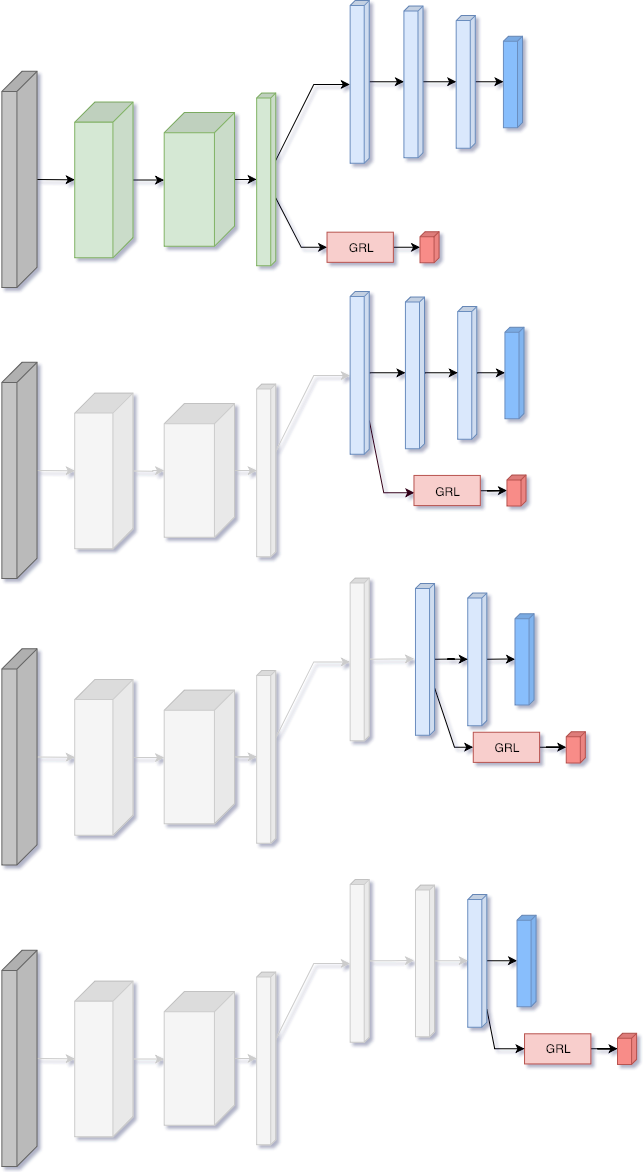
\includegraphics[scale=0.45]{domain_v.png}%
    \caption{Filtering out the domain information process. Firstly the domain predictor is plugged to the output of $G_{f}$. Then $G_{f}$ is frozen and a model with GRL is applied to the consecutive layers of class predictor. All previous layers are frozen. Green blocks represent $G_{f}$, blue ones $G_{y}$ while pink are domain predictor $G_{d}$. Grey blocks are frozen layers. Best viewed in color.}
    \label{fig:domain_v}%    
\end{figure}

\par 
 Figure~\ref{fig:domain_v} presents the described learning process. The first layer of $G_{y}$ was frozen and GRL was plugged to the following layer. The process was repeated until the output layer of $G_{y}$, as its values are probabilities of each digit, so measuring the domain information or applying GRL to the model's output would be pointless. Table~\ref{tab:domain_vanishing} shows the classifiers results on each stage. A special, deeper architecture of the class predictor was used during this experiment, what allowed us to monitor the vanishing of the domain information more precisely.
\par
The experiment was repeated on a smaller model with just a single hidden layer, as it was able to reach better accuracy on the test set than the deeper network. Table~\ref{tab:domain_v_single_hidden} presents detailed results. Obtained model's score is better than the score of the basic model, so a small improvement was made.

\begin{table}[!htbp]
\centering
\begin{adjustbox}{width=1.2\textwidth,center=\textwidth}
\begin{tabular}{c|c|c|c}
\multicolumn{1}{l}{} & \multicolumn{1}{l}{} & \multicolumn{1}{l}{} & \\
Accuracy of \textbackslash{} model's layer & $G_{f}$ output & $G_{y}$ 1st layer & $G_{y}$ 2nd layer \\ 
\hline
Domain classifier on output & 99.99\%~ & 89.69\% & 77.43\%  \\ 
\hline
Domain classifier after adding GRL~ & 93.95\% & 78.28\% & 71.83\%  \\ 
\hline
\begin{tabular}[c]{@{}l@{}}Target domain test set classification \\(after applying domain predictor with GRL)\end{tabular} & 76.91\% & 80.6\% & 80.7\%  
\end{tabular}
\end{adjustbox}
\caption{Filtering out the domain information for $G_{y}$ with a single hidden layer. The information about the sample distribution is progressively removed by domain predictors with GRL.}
\label{tab:domain_v_single_hidden}
\end{table}

\par
Adding a domain classifier with GRL definitely caused the decay of distribution information in the layers of class predictor. Therefore, the output of consecutive $G_{y}$ layers is more domain invariant. We can also notice, that in deeper layers of the model, the decrease of domain predictor accuracy was small. It seems like applying an extra domain classifier is more reasonable on early layers of $G_{y}$. It may be helpful observation, if the learning process lasts for a long time. To sum up, filtering out the domain features from more than one layer in the whole model is a successful modification.


\section{Hyperparameters impact}

\subsection{Training continuation with increased $\lambda$}
During the training process the $\lambda$ coefficient grows from 0 to 1, as the feature extractor's output should be firstly adjusted to a label predictor, and then made more and more domain invariant. When the final model is obtained, parameters $\Theta_{y}$ are well tuned, as the accuracy on source domain is high, the only limitation is not domain invariant enough transformation made by $G_{f}$. Therefore we could try to increase the $G_{d}$ impact, when $G_{y}$ is already well trained. The learning process was repeated with a single modification - $\lambda$ had fixed value, that was greater than 1. In first attempt $\lambda$ was set to 3. After a short training on \mnist the model had 79.2\% accuracy on MNIST-M test set. Then the $\lambda$ was set to 3 for the consecutive epochs and the result increased to 80.6\%. The result of basic model trained for the same time is very similar, however it seems reasonable to apply this kind of continuation, when larger epochs number does not help.
\par
Setting $\lambda$ parameter to some value grater then 1 is enhancing the impact of domain predictor on feature extractor mapping. If the coefficient would be too large, it may lead to deprecation of the model. During experiments, when $\lambda = 6$ a pre-trained model gets chaotic and does not reach the level from first training. Therefore we should worry about picking the right value for $\lambda$ coefficient during the training continuation.

\subsection{Tuning feature vector size}
As previously verified, the feature vector $f$ is not domain shift invariant. During all the experiments made, $f$ was 320-dimensional. Maybe the size is so large, that $G_{y}$ uses only its fraction, and the rest of the space is filled with valuable information for a distribution predictor. Therefore a smaller size of $G_{f}$ output should be considered.
\par
The intuition is that there may be an optimal size of the feature extractor output. It would be large enough for $G_{y}$ to predict the input's label, but the space left would be too little to be sufficient for any domain predictor. The approach with a domain classifier without GRL should also be tried. If two models would compete for the space of a small feature vector $f$, the feature extractor could be forced to separate the data valuable for each of classifiers.
\par
So far feature extractor was constructed with only convolution layers. During these experiments it was extended by single fully connected layer that was mapping the output from $\mathbb{R}^{320}$ to $\mathbb{R}^{D'}$, where $D' = 280, 240, 200, 180, 160, 120$. Then the smaller feature vector was classified by class predictor $G_{y}$ and domain predictor $G_{d}$ with GRL. 
\par
When $G_{f}$ tries to store all the features in a smaller vector, the training process gets noisy. If the dimensionality $D'$ is too little, the value of the loss function may become NaN. As $G_{f}$ returns just few values, both predictors compete for significant changes in most of them, what lead to the failure of the training.
\par
After each architecture's training on \mnist the results were not special at all. The more complex the model was, the higher accuracy it reached. Moreover, adding a fully connected layer caused a noticeable decrease of the performance. Figure~\ref{fig:size_tune} presents the accuracy of each learned model. 
\begin{figure}[htb]%
    \centering
    \includegraphics[width=\linewidth]{size_tune.png}%
    \caption{Accuracy of models with different feature extractor output size over the epochs. Model with feature extractor output size $D'=320$ has no additional fully connected layer. Other architectures are build with feature extractor extended with single fully connected layer, which return a feature vector $f \in \mathbb{R}^{D'}$. Labels present results on MNIST-M test set. }
    \label{fig:size_tune}%
\end{figure}
\par
In the second tested approach, when $G_{d}$ did not have a gradient reversal layer, the feature extractor tried to return an output clear for both label and domain predictors. If it was too small, the $G_{f}$ could separate the digit and domain features, as they would not fit in together.
\par
The results of such multitasking approach were terrible. The classifiers performed well within their tasks, but accuracy on MNIST-M test-set was under 20\%, more than twice less than a simple CNN trained on MNIST. Figure~\ref{fig:size_nogrl} presents the results for different dimensionality of feature vector $f \in \mathbb{R}^{D'}$.
\begin{figure}[htb]%
    \centering
    \includegraphics[width=\linewidth]{sizenogrl.png}%
    \caption{Accuracy of models with different feature extractor output size over the epochs. During the training domain predictor did not contain GRL. This kind of training led to the huge decrease of model's accuracy.}
    \label{fig:size_nogrl}%
\end{figure}
\par
Limiting the feature vector size did not force the feature extractor to separate the data. It seems that domain predictor's impact on feature extractor is so high, that the $G_{f}$ mapping becomes highly correlated with the input distribution. Therefore, when we transform a sample from the target domain, its representation is meaningless. Straightforward using of a common feature extractor is not a good idea then.

\section{Impact of gradient modifications}
Since domain information remains in feature vector, the real effect of GRL should be considered. Adding random noise is one of the gradient modifications that regularize the network \cite{noise}. Therefore, GRL itself could also be some kind of a regularization. With the following experiments we try to check, how complex the effect of GRL is, by comparing its results with some other gradient modifications.
\par
Each of the following modifications were placed at the beginning of the domain predictor and used only during backpropagation pass, just like the transformation made by the gradient reversal layer. Experiments were made on \mnist domains.

\subsection{Random gradient replacement}
First of tested gradient modifications was replacing the real gradient with some random numbers from range $(-1,1)$ multiplied by $\lambda$ parameter. If the results of obtained model were similar to the accuracy of the network with GRL, the gradient reversal layer could be seen as a very simple regularization, that adds some random noise to the gradient of the classifier. It would be equal then to use the domain predictor with GRL, as to apply the approach from mentioned paper \cite{noise}.
\par
At the very beginning of the training, the loss function became NaN. It could be caused by the magnitude of the random number, therefore the range of the random value was limited to $(-\frac{1}{10}, \frac{1}{10})$, but the failure repeated. It was needed to limit the new gradient value to $(-\frac{1}{10000}, \frac{1}{10000})$ to finish the learning process. However, with such a low value, the $G_{d}$ impact on the feature extractor was insignificant. The obtained model was performing like a basic digit classifier. The $G_{d}$ reached very high accuracy in domain predicting, as there was nothing that would disturb it, its gradient was ignored by the feature extractor.
\par
Replacing gradient by some random values does not seem very effective. Firstly, the random value must be small, otherwise, the training fails. Secondly there is not any improvement of the model. Performance of the obtained model is far from the network with GRL, therefore the gradient reversal layer is something more complex than such a simple regularization. 

\subsection{Random sign inversion}
As the GRL usage is not a simple added noise, the values of domain predictor's gradient are crucial to tune the parameters. We can test then, if it is necessary to change the sign of every value. The new modification could be then multiplying only fraction of gradient's value by $-\lambda$, and the rest by $\lambda$.
\par
After the training the model's performance was very close to the network with GRL. Accuracy on source domain reached 98.58\%, and samples from target distribution were classified well in 77.76\%. The domain predictor, with first layer that was modifying the gradient in described way, managed to predict well the distribution of 69.58\% samples. Table~\ref{tab:grad_mod} presents the results of this and following tested modifications.
\par
Multiplying just a fraction of gradient's values by a negative number causes comparable improvement to the GRL, which inverts the sign of every value. Therefore the advance of GRL may be caused by just changing the direction of the optimization step. It is not necessary then to follow exactly the opposite direction to the $G_{d}$ loss gradient. 

\subsection{Random gradient multiplying}
We already know that it is not needfully to multiply each of gradient values by a negative $\lambda$ coefficient. Now we can check how important is to use equal $\lambda$ for all parameters and keep the relative magnitude of these values. Therefore, the next gradient transformation could be multiplying it by some random numbers from range $(-1, 1)$. The increasing $\lambda$ coefficient is not needed anymore. With such transformation not only a fraction of values change their sign, but their significance may be changed. 
\par
The gradient value is considerably different from the origin after the modification, therefore this model could perform comparably to the random gradient replacement. However, the results are even closer to the GRL model, than in the random sign inversion experiment. The accuracy on source domain was 98.75\% and the score on target distribution was 79.12\%. This result is very similar to the accuracy of the model with GRL trained for the same time. Table~\ref{tab:grad_mod} presents the result in comparison to others gradient modifications.
\par
Inverting the sign of a fraction of gradient's values and changing their relative magnitude is a modification with very comparable effect to the GRL. Therefore, it is enough to modify the gradient much more randomly. With this transformation, the optimization step has its size and direction significantly changed. The advantage of the GRL may be then just avoiding the step in the direction of the domain predictor loss gradient.

\begin{table}
\centering
\begin{adjustbox}{width=1.2\textwidth,center=\textwidth}
\begin{tabular}{c|c|c|c|c}

\multicolumn{1}{l}{} & \multicolumn{1}{l}{} & \multicolumn{1}{l}{} & \multicolumn{1}{l}{} & \\ & GRL & \begin{tabular}[c]{@{}c@{}}Random sign\\inversion\end{tabular} & \begin{tabular}[c]{@{}c@{}}Random\\multiplication\end{tabular} & \begin{tabular}[c]{@{}c@{}}Gradient \\Inverse\end{tabular} \\ 
\hline
Accuracy on source domain & 99.12\% & 98.58\%~ & 98.75\% & 98.38\% \\ 
\hline
Accuracy of domain classifier & 67.29\% & 70.49\% & 68.27\%  & 59.28\% \\ 
\hline
Accuracy on target domain & 80.57\% & 77.76\% & 79.12\%  & 78.87\%                                                    
\end{tabular}
\end{adjustbox}
\caption{Results of applying different gradient modifications during backpropagation in \mnist case. The scores are very close to the accuracy of the model with GRL, therefore the advance of the GRL may be just avoiding the parameters update in the direction of the $G_{d}$ loss minimum. The low accuracy of domain predictor when gradient inverse layer was used shows that this method may produce much more domain invariant feature vectors.}
\label{tab:grad_mod}
\end{table}


\subsection{Gradient inversion layer}

The gradient not only points at the direction of the function's minimum, but also determines the magnitude of each parameter's impact on the final result, as gradient is a multi-variable derivative. Therefore, when the goal is to set such parameters $\Theta_{f}$, that the transformation made by $G_{f}$ is absolutely meaningless for the domain predictor, reversing the relative magnitude of gradient's value should be considered. The next transformation could then take the vector of gradient's value, and change the parameters with a small absolute value to a big ones and vice versa. 
\par
This transformation could cause that crucial for $G_{d}$ changes of $\Theta_{f}$ parameters would be ignored, while parameters that were already well tuned from domain predictor point of view, would be significantly changed. Moreover each value would had its sign changed, so the direction of the optimization step is even more changed.
\par
Such modification could disallow the domain predictor from finding any dependencies. If only $G_{d}$ finds any pattern in some $G_{f}$ parameters, they are changed much more than some irrelevant ones, so no meaningful information about domain would occur in feature extractor mapping. 
\par
The described modification takes a vector of gradient's values $x = [x_{0}...x_{D-1}]$ and transforms it to $-\lambda \cdot (\max_{0 \leq i < D} |x_{i}| \cdot sign(x) \dotdiv x)$, where $\dotdiv$ is element-wise difference. Each value of the vector $x$ is subtracted from the largest absolute value from the entire vector multiplied by the $sign(x)$, so the sign of $x$ is kept until $-\lambda$ multiplication.
\par
Accuracy of a model with such transformation placed at the beginning of the domain predictor $G_{d}$ was comparable to previous modifications - it classified well 98.38\% of samples from source domain and 78.87\% from target distribution. The result of domain predictor was much lower - $G_{d}$ score was just 59.28\%. The last column of table~\ref{tab:grad_mod} presents the model's accuracy.
\par
The obtained feature vectors were much more domain invariant than in previous case, at least for the domain predictor used during the learning process. Therefore, the success of this approach shows that some significantly different from GRL gradient modifications should be considered in the domain adaptation.

\section{Other experiments}
\subsection{Measuring orthogonality}
The GRL is used to obtain a feature vector $f$ that contains only the information valuable for the class predictor $G_{y}$, and no features required by domain classifier $G_{d}$. Therefore we want $G_{y}$ and $G_{d}$ to use disjoint sets of data dependencies. Transformation made by each of the classifiers is in fact a matrix multiplication. Feature extractor $G_{f}$ maps the input to vector $f \in \mathbb{R}^{D}$. Predictors contain an input layer, that maps $f \in \mathbb{R}^{D}$ to some $f_{i} \in \mathbb{R}^{I}$. Multiplying the coordinates of D-dimensional point by some matrix is in fact reducing its dimensionality by projecting it onto some directions. 
\par
We can say then, that using disjoint dependencies is in fact transforming the input point with some pairwise (between predictors) orthogonal vectors. Shifting the domain is therefore moving the data along directions that are used by the domain predictor, which would be unnoticeable for class predictor. If feature vector $f$ would contain only features used by class predictor, such move would not change its values. 
\par
We can measure the orthogonality of the vectors used by the predictors, as they are defined by the matrix $D \times I$ of each classifier input layer. If dot product of both matrices it is close to zero, the directions are more orthogonal. When we compute it after the training, it turns out to be a very small number. Therefore directions of $G_{y}$ and $G_{d}$ are almost orthogonal.
\par
We can force the predictors to use even more orthogonal vectors by adding to the objective the mean value of the squared dot product, i.e. if we denote the model loss function as $L(\Theta_{f}, \Theta_{y}, \Theta_{d})$ and classifiers input layer matrices as $W_{I_{y}}$ and $W_{I_{d}}$, then new loss function is:
\begin{equation*}
L'(\Theta_{f}, \Theta_{y}, \Theta_{d}) = L(\Theta_{f}, \Theta_{y}, \Theta_{d}) + \overline{(W_{I_{y}} \cdot W_{I_{d}}^{T})^{2}}
\end{equation*}
\par
The new loss function caused reducing the dot product indeed, but it had no impact on model's performance, therefore GRL itself force the predictors to use as disjoint sets of feature vector dependencies as possible. As the new loss is punishing for product of model's weights, the optimizer may force them to decay. This would be undesirable, we want the dot product to reduce not because of shorter vectors, but because of their orthogonality. However, monitoring the matrices weights shows that there is no shrinking. 

\subsection{Adam Optimizer}
Ganin and Lempitsky used Stochastic gradient descent (SGD) optimizer during their research. However, in recent years some fancy optimization methods released and they can boost the training process even more. One of them is Adam Optimizer \cite{adam}. It is much more complex than SGD, with individual learning rate for each parameter and usage of more gradient's properties. 
\par
To check if Adam may improve our model, the optimizer for each network was changed. After the training, the accuracy on target domain was slightly higher than before. The learning process was repeated few times and after every iteration the highest score was reached by model tuned with Adam, so it turned out to be a good choice. Its parameters should be initialized carefully, as during the training the loss may get NaN value much easier. In our particular case, the initial learning rate was reduced from 0.01 for SGD to 0.001 for Adam.

\section{Cloud point shape analysis and visualizations}
\subsection{Conceptors}
As previously mentioned, feature vectors for all the samples from both domains can be considered as two point clouds $F_{S}$ and $F_{T}$, that can be approximated with ellipsoids. These ellipsoids are described by the conceptors matrices $C_{S}$ and $C_{T}$. The quality of the feature extractor $G_{f}$ mapping may be measured as the similarity of ellipsoids approximating $F_{S}$ and $F_{T}$, as a domain invariant transformation produces the same point cloud for both distributions. Measuring the similarity of $F_{S}$ and $F_{T}$ can be done by conceptors comparison. 
\par
As a conceptor ellipsoid always lies inside an unit sphere, it can be measured, how much of space does it occupies. If the point cloud is scattered over the whole space then it would not be possible to approximate it with nothing but a sphere. However, if points are located in an organized cluster, they can be captured with much more limited ellipsoid. Therefore, the \textit{quota} value measures the fraction of the space that is taken by a conceptor. It can be computed as:
\begin{equation*}
    Q(C) = \frac{1}{N} \sum_{i=1}^{N}{s_{i}}
\end{equation*}
where $s_{i}$ are singular values of the conceptor matrix $C$. Moreover, logic operations  can be applied to the conceptors, such as $\neg, \vee, \wedge$. The negation of conceptor is the space orthogonal to the ellipsoid. The disjunction is a conceptor that is obtained with a sum of samples sets approximated by two conceptors, while the conjunction is the conceptor that approximates the intersection of these sets. Figure~\ref{fig:conceptor_logic} charts these operations.
\begin{figure}%
    \centering
    \includegraphics[width=\linewidth]{c_logic.png}%
    \caption{Logic operations on 2-dimensional conceptors. Picture from \cite{overc}.}
    \label{fig:conceptor_logic}%
\end{figure}
\par
To assess the similarity of two point clouds, corresponding conceptors $C_{S}$ and $C_{T}$ should be computed firstly. Then $C_{S} \vee C_{T}$ is their intersection. The value $Q(C_{S} \vee C_{T})$ determines its magnitude. If it is close to both $Q(C_{S})$ and $Q(C_{T})$ then ellipsoids that approximate both point clouds are similar. The quota of conjunction $Q(C_{S} \wedge C_{T})$ should also be close to the $Q(C_{S} \vee C_{T})$, as intersection of these point clouds should include most of them.
\par
Reliable result demands well computed conceptors. The final values of matrix $C$ depend on the magnitude of the scaling parameter $\alpha$, called the aperture. If it is too low, the conceptor acts as zero mapping, while when the aperture is getting larger, the conceptor matrix becomes an identity matrix.
\par
The proper aperture value could be taken from the paper published by Xu He and Herbert Jaeger "Overcoming Catastrophic Interference using Conceptor-Aided Backpropagation" \cite{overc}, where conceptors are used to learn MNIST and its permutations. Authors try to obtain a model that performs well on following datasets and conceptors are used to determine the ability of the model to learn a new MNIST permutation and the still spare space, so the next task could fit there. When quota of the concpetor that approximate the already taken space gets 1, capacity of the network is full and trying to fit any other dataset fails.
\par
As MNIST was the main dataset in the paper and received results were satisfying, it seems reasonable to use the same $\alpha$ as the authors and try to measure the similarity of $F_{S}$ and $F_{T}$ point clouds in \mnist case. Therefore, conceptor matrices \CM $\in \mathbb{R}^{D\times D}$ and \CMM $\in \mathbb{R}^{D\times D}$ were computed with $\alpha = 4$, as that value was used in most experiments in the paper. The conceptors were approximating feature vectors $f \in \mathbb{R}^{D}$ for all samples from both distributions.
\par
When quota values were measured, both of them were over $0.99$. This was highly undesirable, as it implied that the points form both point clouds were scattered over the space, therefore the ellipsoids approximating them were not a good depiction. Even the value $Q$(\CM $\vee$ \CMM) and $Q$(\CM $\wedge$ \CMM) were close to each other and to quotas of each conceptors, it did not mean the $F_{MNIST}$ and $F_{MNIST-M}$ were similar. We could only conclude that points from these cloud lied in many regions of the space. 
\par
For any $\alpha > 1$ the quota of conceptor was over $0.99$, to obtain $Q$(\CM) < 0.9 it was needed to set $\alpha = 0.4$. With such a low aperture it is hard to say if the results are reliable. However, for all tested values, the $Q$(\CM) and $Q$(\CMM) were close.
\par
When model was trained without a domain predictor with GRL, the $Q$(\CM) was as high as previously, but the quota of \CMM \ was significantly lower. As $F_{MNIST-M}$ may be captured with a smaller ellipsoid, then it must be different from $F_{MNIST}$. Figure~\ref{fig:Q(C)} presents the quota values of \CM \ and \CMM when aperture was in range $[0.1, 1]$.

\begin{figure}
    \centering
    \begin{subfigure}[b]{0.48\textwidth}
        \includegraphics[width =\textwidth]{Q(C).png}
        \caption{Model trained with GRL}
    \end{subfigure}%
    \begin{subfigure}[b]{0.48\textwidth}
        \includegraphics[width =\textwidth]{Q(C_nogrl).png}
        \caption{Model trained without GRL}
    \end{subfigure}%        
    \caption{Quota of concpetors \CM (blue) and \CMM (green) for training with or without domain predictor with GRL.}%
    \label{fig:Q(C)}%
\end{figure}
\par
Jaeger proposes conceptors as a way to transform a given point into a point cloud that is well known by the model \cite{conc}. This idea sounds attractive for domain adaptation. After computing the conceptor $C_{S}$ for data cloud $F_{S}$, while input sample $x$ would be classified, its feature vector $f = G_{f}(x ; \Theta_{f})$ could be multiplied by $C_{S}$ before processing by class predictor $G_{y}$. This would project it into data cloud that is already well known for the label predictor. Therefore the probabilities for each class would be computed as:
\begin{equation*}
  P(x) =  G_{y}( G_{f}( x ; \Theta_{f} ) \cdot C_{S} ; \Theta_{y} )    
\end{equation*}
Even though this approach was successful with echo-state network \cite{conc}, it did not improve the trained model's performance. The $F_{S}$ and $F_{T}$ point clouds were probably similar enough to had almost equal conceptor matrices, therefore multiplying a point form $F_{T}$ by $C_{S}$ was close to identical mapping. Therefore, using conceptors for model's improvement was ineffective.

\subsection{Visualization}
Comparing the $F_{S}$ and $F_{T}$ did not succeed with the conceptors. The knowledge about these point clouds could be helpful in understanding the problem of domain adaptation as well as the gradient reversal layer effect. Therefore we could try to visualize them by setting the size of feature extractor to 3. The $G_{f}$ mapping would be then a function $\mathbb{R}^{M} \rightarrow \mathbb{R}^{3}$, where M is the dimensionality of input sample $x$. Such mapping can be obtained by extending the original feature vector by a single fully connected layer that transforms the feature vector $f \in \mathbb{R}^{D}$ to $\mathbb{R}^{3}$. This kind of feature extractor may be denoted as $G_{3}$ with parameters $\Theta_{3}$. When each point in $F_{S}$ and $F_{T}$ is a 3-dimensional feature vector, its values may be treated as the coordinates, so the point cloud can be easily drawn.
\subsection{MNIST and MNIST-M visualizations}
Training a model with such a small layer inside is much more difficult task, as many information may be lost during mapping do $\mathbb{R}^{3}$. Therefore, at the beginning the domain classifier $G_{d}$ with GRL was not used. The point clouds in \mnist case might be denoted as $F_{MNIST}$ and $F_{MNIST-M}$. The model achieved 98\% accuracy on the MNSIT test set, but it performed poorly on MNIST-M, just 31\% of digits, were classified well. As parameters of $G_{3}$ were tuned, the point clouds could be visualized. Figure~\ref{fig:MNIST_3D}(a) shows the result of mapping by $G_{3}$ all the samples from MNIST test set (blue) and MNIST-M test set (gray). The shape of both point clouds resemble a multi-armed star. Moreover it seems like $F_{MNIST}$ is just a stretched version of $F_{MNIST-M}$. We can expect that each arm contains mapped pictures of same digit. Figure~\ref{fig:MNIST_3D}(b) presents distribution of the images of zero digit from both domains. In both cases the pictures transformations form corresponding arm of the star.
\par
\begin{figure}[htb]%
    \centering
    \begin{subfigure}[b]{0.48\textwidth}
        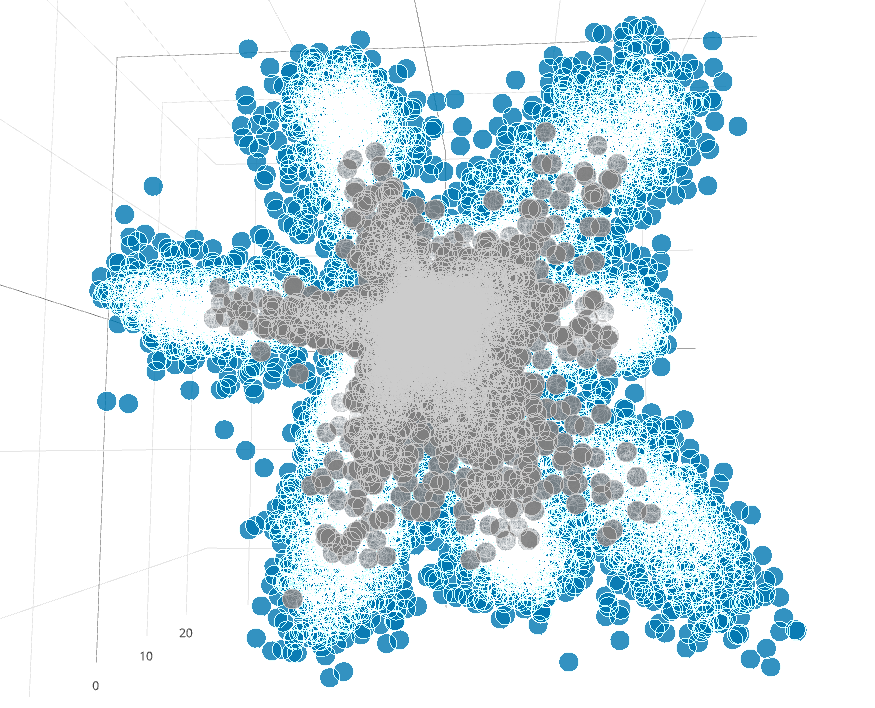
\includegraphics[width =\textwidth]{MNIST_MNISTM.png}
        \caption{MNIST and MNIST-M}
    \end{subfigure}%
    \begin{subfigure}[b]{0.48\textwidth}
        \includegraphics[width =\textwidth]{Zeros_MNIST_MNISTM.png}
        \caption{Zero digit samples}
    \end{subfigure}%    
    \caption{The visualization of samples transformed by feature extractor $G_{3}$. (a) presents two stars formed by samples from source domain (MNIST/blue) and a target domain (MNIST-M/gray) (b) shows how pictures of zero digit are mapped - yellow points are zeros from MNIST and green ones from MNIST-M}%
    \label{fig:MNIST_3D}%
\end{figure}

\subsection{GRL visualizations}
As the previous visualization shown, $F_{S}$ and $F_{T}$ are quite similar. It could be expected, that learning the model with GRL should make these point clouds even closer. The next model was composed with feature extractor $G_{3}$, label predictor $G_{y}$, and domain classifier $G_{d}$ with GRL. After the training the model got 96\% accuracy on source domain test set and 40\% accuracy on target domain test set. The improvement was almost 30\% in relation to the model without GRL.
\par
The visualization of both point clouds mapped by $G_{3}$ is really surprising.  Figure~\ref{fig:GRL3D} shows how samples from source and target domain were transformed. The second picture presents samples from both distributions. The target domain point cloud $F_{MNIST-M}$ formed a blob that is not similar to the source domain distribution $F_{MNIST}$ at all. The last picture shows the location of zero digit images.

\begin{figure}[htb]%
    \centering
    \begin{subfigure}[b]{0.33\textwidth}
        \includegraphics[width =\textwidth]{GRL_3D1.png}
    \end{subfigure}%
    \begin{subfigure}[b]{0.33\textwidth}
        \includegraphics[width =\textwidth]{GRL_3D2.png}
    \end{subfigure}%
    \begin{subfigure}[b]{0.33\textwidth}
        \includegraphics[width =\textwidth]{GRL_3D3.png}
    \end{subfigure}%   
    
    \caption{Output of $G_{3}$ mapping when GRL was used during training. First picture presents how source domain samples are transformed, second one shows the point clouds for both source (blue) and target (gray) domain. Last picture shows how points with 0 label are distributed.}%
    \label{fig:GRL3D}%
\end{figure}
\par
Training process is very noisy, when feature extractor output is so small. The results after different runs were very diverse. The training often failed when the loss became NaN, the variance of model's accuracy over training was high. Mapping the feature vector to just 3 numbers caused the loss of many information. Therefore, to avoid the failure of training process, the $\lambda$ was set to fixed value $\lambda = 0.3$. This allowed the model to perform better, the accuracy on MNIST-M test set was over 50\%.

\begin{figure}%
    \centering
    
    \begin{subfigure}[b]{0.33\textwidth}
        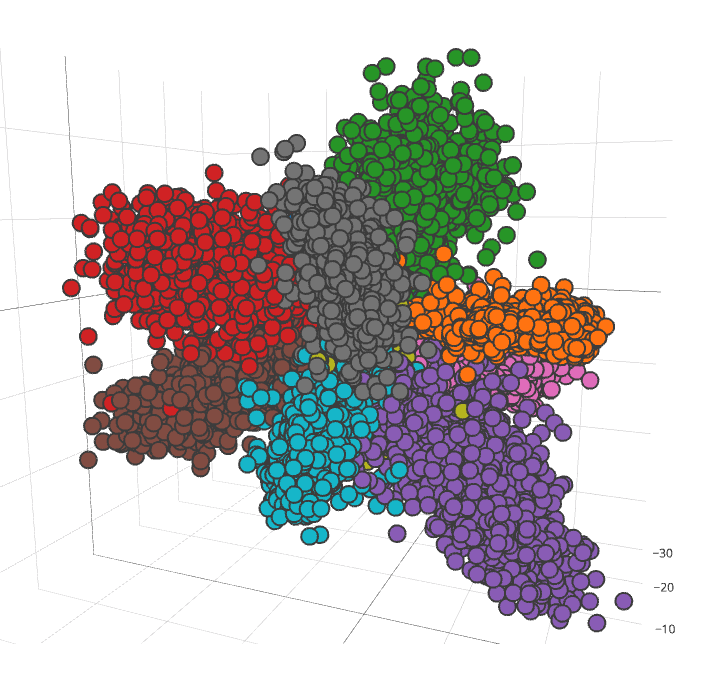
\includegraphics[width =\textwidth]{GRL_digits1.png}
        \caption{$F_{MNIST}$}
    \end{subfigure}%
    \begin{subfigure}[b]{0.33\textwidth}
        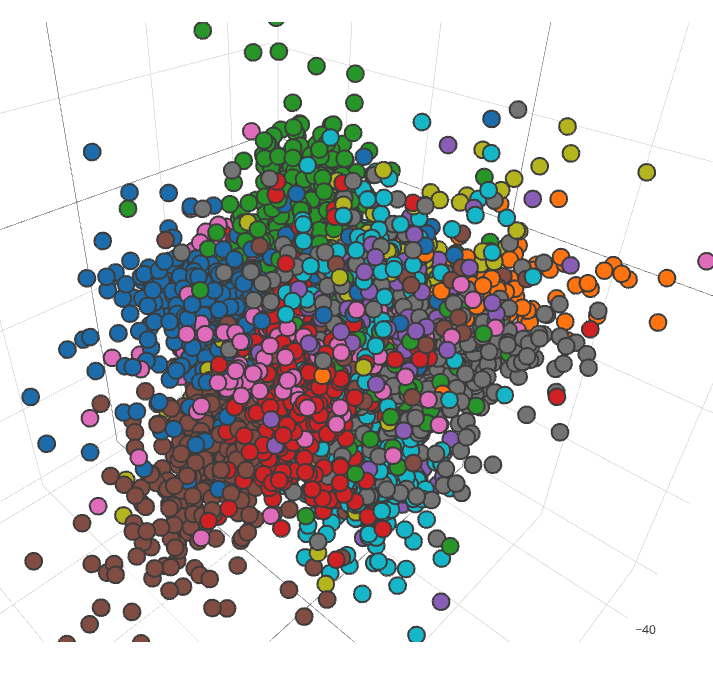
\includegraphics[width =\textwidth]{GRL_digits2.png}
        \caption{$F_{MNIST-M}$}
    \end{subfigure}%
    \begin{subfigure}[b]{0.33\textwidth}
        \includegraphics[width =\textwidth]{GRL_digits3.png}
        \caption{Both point clouds}
    \end{subfigure}%

    \caption{Mapping of the input images of particular digits. The model was learned with GRL and fixed value $\lambda = 0.3$}%
    \label{fig:GRL_digits}%
\end{figure}

\par
To make the plots even more understandable, the feature vector may returns a 2-dimensional feature vector $f \in \mathbb{R}^{2}$. Figure~\ref{fig:2D} presents the $F_{MNIST}$ and $F_{MNIST-M}$ mapped to $\mathbb{R}^{2}$ with and without using the GRL. Without the GRL, the point clouds formed multi-armed stars again. Each star has less arms than number of classes in the dataset, therefore few of them are stacked in the middle. Classifying of these samples is likely much less accurate. Moreover, majority of points from $F_{MNIST-M}$ lies close to the middle of the coordinate system. As input images of different digits are represented by similar numbers, the classifier cannot be sure while predicting their label. When GRL was applied during the training, the accuracy on the MNIST-M was much higher, but the samples formed a blob, therefore the better performance is incomprehensible. 

\begin{figure}[htb]%
    \centering
    
    \begin{subfigure}[b]{0.33\textwidth}
        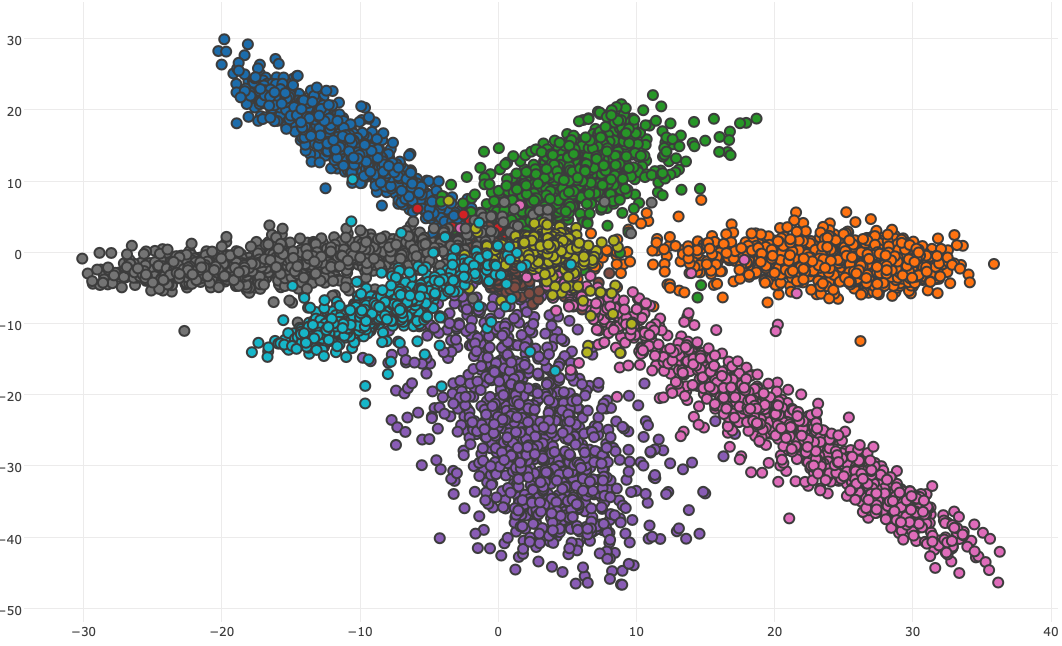
\includegraphics[width =\textwidth]{MNIST_2D.png}
    \end{subfigure}%
    \begin{subfigure}[b]{0.33\textwidth}
        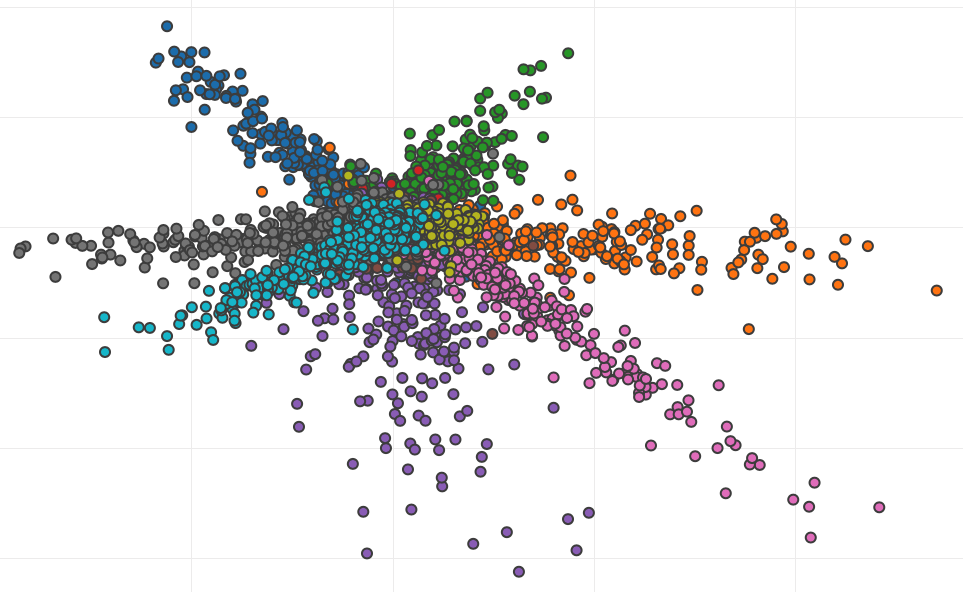
\includegraphics[width =\textwidth]{MNIST_M_2D.png}
    \end{subfigure}%
    \begin{subfigure}[b]{0.33\textwidth}
        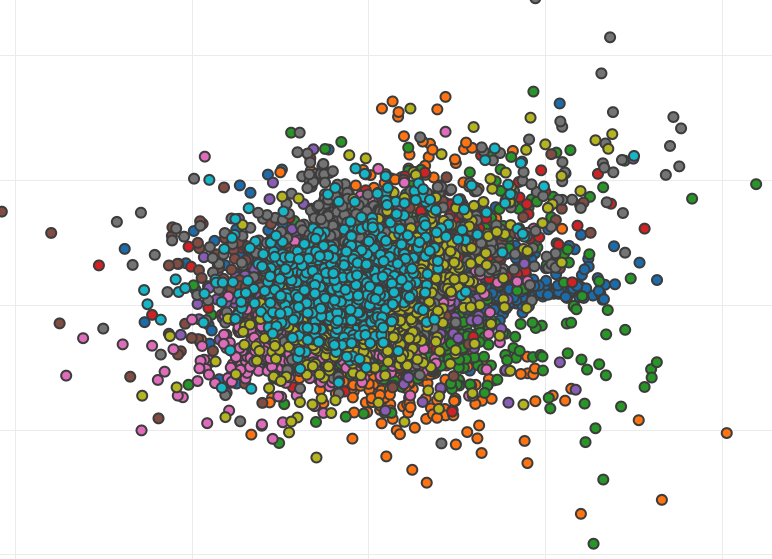
\includegraphics[width =\textwidth]{MNIST_M_2D_GRL.png}
    \end{subfigure}%   
    
    \caption{2-dimensional feature vector mapping. First picture shows the distribution of samples from source domain, second one presents the $F_{MNIST-M}$ without applying GRL during training, while the last image shows $F_{MNIST-M}$ when GRL was used.}%
    \label{fig:2D}%
\end{figure}

\subsection{SVHN visualizations}
\par
In \svhn case, visualizing the point cloud $F_{SVHN}$ formed by samples from SVHN dataset mapped by feature vector $G_{3}$ is much more challenging. SVHN images are more complex, so compressing the information required to a good classification into just 3 values is a tough mission. Fortunately, a model with a complex $G_{3}$ architecture reached 92\% accuracy on the SVHN test set and 65\% on target domain (MNIST) samples. The performance on MNIST test set is satisfying, the majority of the information was not lost during mapping to $\mathbb{R}^{3}$. Figure~\ref{fig:SVHN_Digits} presents the visualization of $F_{SVHN}$ and $F_{MNIST}$ after mapping by $G_{3}$.
\par
The point clouds are much more similar this time, what is related to the better performance of the model on target domain. 
Also images of every digit from SVHN formed a sharp, individual arm, while pictures from target domain are a bit mixed, with many of the samples close to the middle of the coordinate system. Therefore classifying a sample by its location in the star formed by the point cloud may be unsuccessful.

\begin{figure}[htb]%
    \centering
    \begin{subfigure}[b]{0.48\textwidth}
        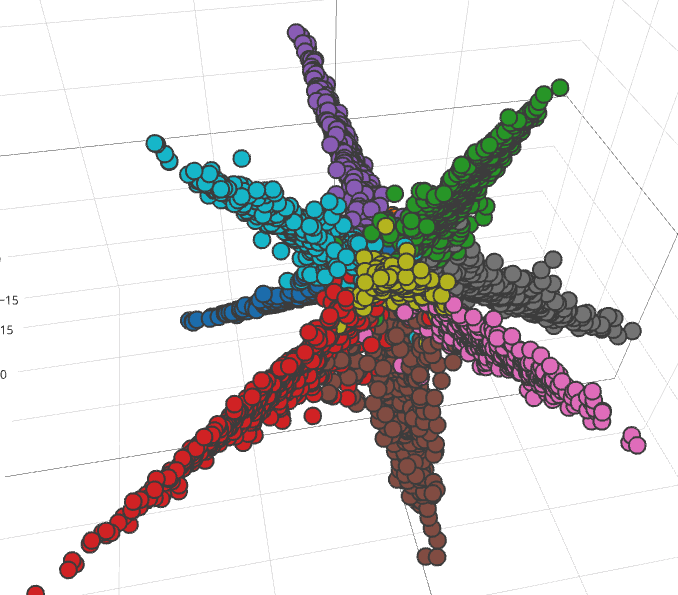
\includegraphics[width =\textwidth]{SVHN_digits1.png}
        \caption{$F_{SVHN}$}
    \end{subfigure}%
    \begin{subfigure}[b]{0.48\textwidth}
        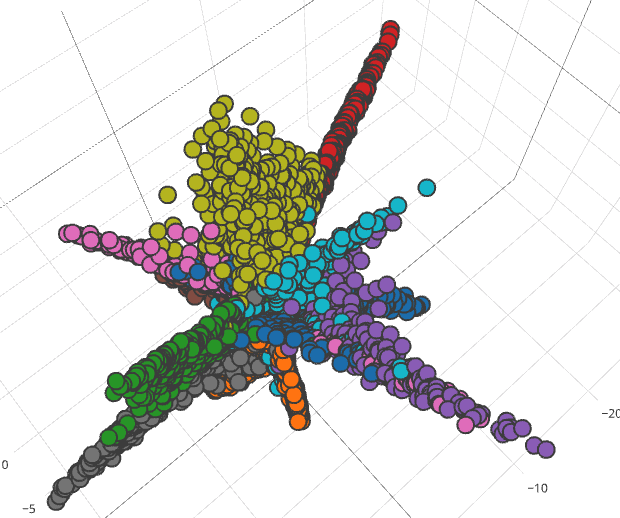
\includegraphics[width =\textwidth]{SVHN_digits2.png}
        \caption{$F_{MNIST}$}
    \end{subfigure}%        
    \caption{Distribution of particular digit images after $G_{3}$ mapping.}%
    \label{fig:SVHN_Digits}%
\end{figure}
\par
Training with GRL applied was already very unstable in \mnist, therefore, it was not surprising that with in \svhn applying GRL during training a fresh model caused the failure of the learning process. Even if $\lambda$ was set to a fixed small value, the loss function became NaN. Nonetheless, the already trained model could be extended with a domain predictor $G_{d}$ with GRL plugged to the output of the feature extractor. After that kind of training, accuracy on SVHN test set was 73\%, therefore applying GRL increased the model's performance by 12\%. $\lambda$ parameter had to be fixed and small to avoid the training failure again. With $\lambda = 0.2$ the model managed to tune its parameters well. Figure~\ref{fig:SVHN_GRL} presents the distribution of both point clouds mapped by $G_{3}$ after the posterior training with GRL applied. This time the target domain samples did not formed a blob, however, the GRL impact on the entire model was much lower in this case. The multi-armed star formed by $F_{SVHN}$ is not as sharp as previously. Also samples from the $F_{MNIST}$ are less mixed, and the point cloud itself is more similar to the $F_{SVHN}$.

\begin{figure}[htb]%
    \centering
    \begin{subfigure}[b]{0.48\textwidth}
        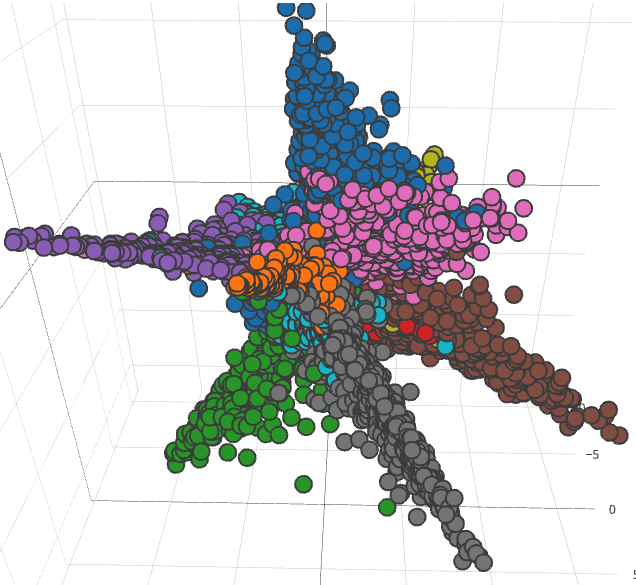
\includegraphics[width =\textwidth]{SVHN_GRL.png}
        \caption{$F_{SVHN}$}
    \end{subfigure}%
    \begin{subfigure}[b]{0.48\textwidth}
        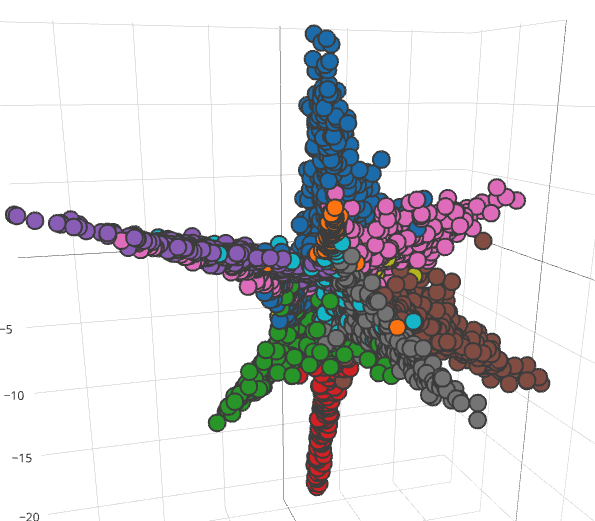
\includegraphics[width =\textwidth]{SVHN_GRL2.png}
        \caption{$F_{MNIST}$}
    \end{subfigure}%        
    \caption{Distribution of particular digit images after $G_{3}$ mapping, when GRL was used during the training.}%
    \label{fig:SVHN_GRL}%
\end{figure}

\subsection{3-dimensional layer in class predictor}
Such a restrictive limitation of the feature vector $f$ dimensionality caused a serious decline of model's performance. Also using the GRL during training was unsettled, as the learning process often failed. Therefore the layer with the output size 3 could be placed in the class predictor, rather than as the last layer of the feature extractor. This approach favours also the training with GRL, as the gradients from both predictors influence a D-dimensional feature vector. The new architecture is then build with feature extractor $G_{f}$ that produces the feature vector $f \in \mathbb{R}^{D}$, domain predictor $G_{d}$ with GRL and the class predictor $G_{y}^{3}$ with a single hidden layer of size 3. 
\par
This architectural change cuased a significant improvement of the model's performance. In \mnist case after a short training, the accuracy on MNIST-M reached 69.08\%, what was much closer to the results obtained by the model with no architectural limitations. To visualize the input sample $x$, it is firstly transformed by $G_{f}$ to feature vector $f \in \mathbb{R}^{D}$ and then mapped by the first layer of class predictor $G_{y}^{3}$ to a 3-dimensional vector $f_{3} \in \mathbb{R}^{3}$. Figure~\ref{fig:vis_class_pred} presents the result of such mapping. Both point clouds again formed multi-armed stars, but they are much more similar in this case. Also applying GRL did not resulted in transformation of the target domain point cloud to a blob. Using $G_{y}^{3}$ instead of $G_{3}$ is definitely a better approach to visualize the data.
\begin{figure}[htb]%
    \centering
    \begin{subfigure}[b]{0.48\textwidth}
        \includegraphics[width =\textwidth]{bv1.png}
        \caption{Point clouds mapped to $\mathbb{R}^{3}$}
    \end{subfigure}%
    \begin{subfigure}[b]{0.48\textwidth}
        \includegraphics[width =\textwidth]{bv2.png}
        \caption{Digits from MNIST mapped to $\mathbb{R}^{3}$}
    \end{subfigure}%   
    \captionsetup{belowskip=0pt}
    \caption{Mapping of $F_{MNIST}$ and $F_{MNIST-M}$ to $\mathbb{R}^{3}$ by class predictor's first layer. First picture presents both point clouds - blue is the mapping of $F_{MNIST}$, gray is $F_{MNIST-M}$. The second image shows the distribution of each digit from MNIST. Once again the mapped sampled formed a multi-armed star.}%
    \label{fig:vis_class_pred}%
\end{figure}
\par
As visualizations with $G_{y}^{3}$ seem more reliable it can be used to some other analysis. As some of the mapped samples are mixed close to the middle of the coordinate system, they are likely wrongly classified. Therefore, the distribution of samples with worst and best prediction could be checked. Figure~\ref{fig:best_pred} presents the location of misclassified samples and the input images that are predicted well with highest score from the model. It confirms that mapping the input into the middle area may cause the mistake during classification.
\begin{figure}[!htbp]%
    \centering
    \begin{subfigure}[b]{0.48\textwidth}
        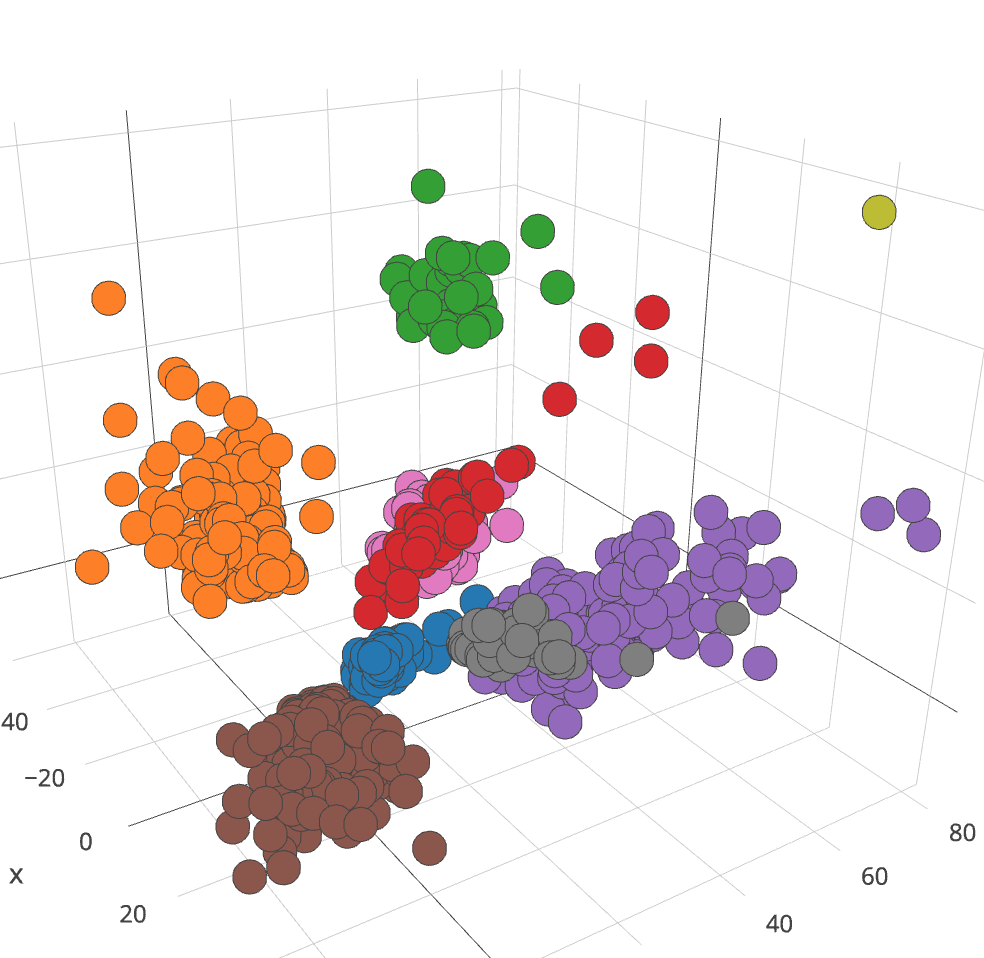
\includegraphics[width =\textwidth]{best_pred1.png}
        \caption{Best predictions}
    \end{subfigure}%
    \begin{subfigure}[b]{0.48\textwidth}
        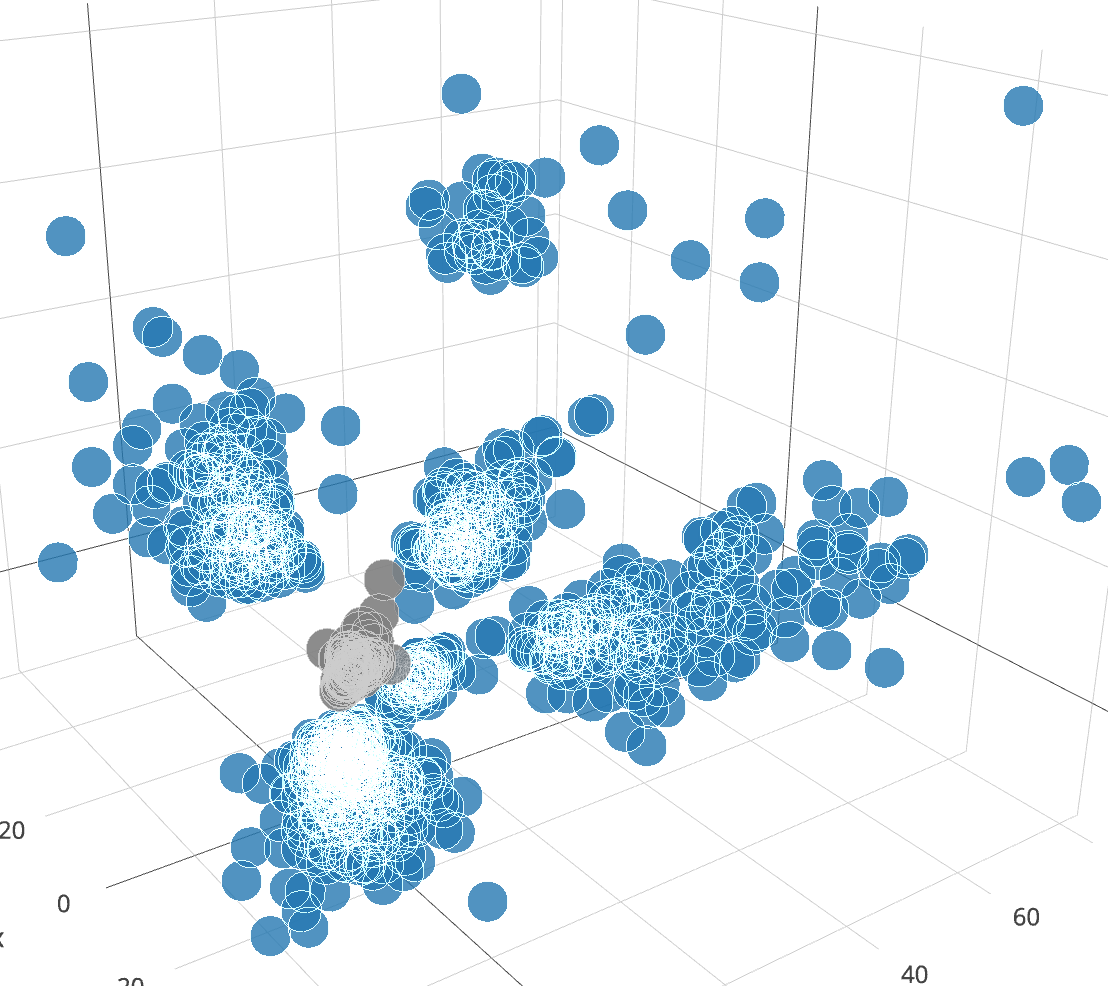
\includegraphics[width =\textwidth]{best_pred2.png}
        \caption{Best and worst predictions}
    \end{subfigure}%        
    \caption{Distribution of best and worst predictions by the model. First picture shows the location of samples that are classified well, with highest score assigned by the model. Second image shows all these samples as blue ones and some of the misclassified samples (gray).}%
    \label{fig:best_pred}%
\end{figure}

\subsection{Visualizations with dimensionality reduction techniques}
Even with 3-dimensional layer in class predictor, forcing the model to use such a small layer causes the decrease of its performance. To avoid this, some of the dimensionality reduction techniques may be used to obtain the representation of the data in $\mathbb{R}^{3}$. One of them is PCA, that transforms the data by projecting them onto the principal vectors of the data points correlation matrix. To obtain best possible approximation of the data, the vectors corresponding to the greatest principal values should be chosen. 
\par
Firstly, the correlation matrix was computed for both $F_{MNIST}$ and $F_{MNIST-M}$. When the singular values of the matrices were computed, the greatest 3 of them were not much greater than many others. It confirms, that the obtaining a good feature extractor demands the dimensionality of feature extractor to be much higher than $\mathbb{R}^{3}$. Therefore, projecting the data onto just 3 vectors caused a huge loss of the information. 
\par
Figure~\ref{fig:dim_red} presents the visualizations of $F_{MNIST}$ and $F_{MNIST-M}$ obtained with PCA and Kernel-PCA with RBF kernel, that firstly transforms the input data to some higher-dimensional space. The results are not as impressive as with 3-dimensional layer in the model. However, it can be clearly seen that applying GRL makes the point clouds much more similar. 

\begin{figure}[!htbp]%
    \centering
    
    \begin{subfigure}[b]{0.33\textwidth}
        \includegraphics[width =\textwidth]{pca_nogrl.png}
        \caption{PCA, without GRL}
    \end{subfigure}%
    \begin{subfigure}[b]{0.33\textwidth}
        \includegraphics[width =\textwidth]{pca_grl.png}
        \caption{PCA, with GRL}
    \end{subfigure}%
    \begin{subfigure}[b]{0.33\textwidth}
        \includegraphics[width =\textwidth]{kpca.png}
        \caption{Kernel-PCA on $F_{MNIST}$}
    \end{subfigure}%
    \caption{The visualizations with dimensionality reduction techniques. First two pictures presents the point clouds for source (blue) and target (gray) domain, transformed to $\mathbb{R}^{3}$ with PCA method. Applying GRL during training results in more similar point clouds. The last picture presents distribution of each digit with Kernel PCA used to reduce the dimensionality.}%
    \label{fig:dim_red}%
\end{figure}

\subsection{Other visualizations}
The well trained feature extractor $G_{3}$ could be used to visualize the transformation made by conceptor. With \mnist distribution, the ellipsoid approximating the $F_{MNIST}$ could be computed and represented as conceptor \CM. The quota $Q$( \CM) value was close to 1 for even very small values of aperture $\alpha$. This seems reasonable, as the obtained multi-armed star cannot be captured with nothing but a sphere. Therefore, the \CM matrix was close to the identity matrix, so multiplying the samples of $F_{MNIST-M}$ by \CM did not make the point cloud more similar to $F_{MNIST}$. Figure~\ref{fig:vconc} presents the result of such transformation.
\begin{figure}[!htpb]%
    \centering
    
    \begin{subfigure}[b]{0.27\textwidth}
        \includegraphics[width =\textwidth]{vconc1.png}
    \end{subfigure}%
    \begin{subfigure}[b]{0.27\textwidth}
        \includegraphics[width =\textwidth]{vconc2.png}
    \end{subfigure}%
    \begin{subfigure}[b]{0.27\textwidth}
        \includegraphics[width =\textwidth]{vconc3.png}
    \end{subfigure}%

    \caption{Transformation the $F_{MNIST-M}$ point cloud woth \CM. First picture shows point clouds $F_{MNIST}$ (blue) and $F_{MNIST-M}$ (gray) obtained after the training (domain predictor with GRL was not used). The second picture presents the transformation of the $F_{MNIST-M}$ point cloud (gray) by conceptor \CM (green). The difference is almost imperceptible. The last picture shows all three point clouds together.}% 
    \label{fig:vconc}%
\end{figure}
\par
The multiplication by conceptor matrix only reduced the area of the point cloud. As every conceptor matrix $C$ is a positive semidefined matrix \cite{conc}, it can be presented as $C = U\Sigma U^{T}$, where $U$ and $U^{T}$ can be interpreted as rotation matrices and $\Sigma$ is a diagonal matrix with singular values of $C$ on diagonal. As all singular values of conceptor matrix are real numbers from range $[0,1]$, the conceptor matrix multiplication is in fact rotation, shortening (as non-zero values of $\Sigma$ are $\leq 1$ \cite{conc}) in certain directions and then re-rotation of the point cloud (see figure~\ref{fig:ConceptorRotation}).

\begin{figure}[!htpb]%
    \centering
    \begin{subfigure}[b]{0.24\textwidth}
        \includegraphics[width =\textwidth]{C1.png}
        \caption{$F_{M}$}
    \end{subfigure}%
    \begin{subfigure}[b]{0.24\textwidth}
        \includegraphics[width =\textwidth]{C2.png}
        \caption{$U^{T} \cdot F_{M}$}
    \end{subfigure}%
    \begin{subfigure}[b]{0.24\textwidth}
        \includegraphics[width =\textwidth]{C3.png}
        \caption{$\Sigma \cdot U^{T} \cdot F_{M}$}
    \end{subfigure}%    
    \begin{subfigure}[b]{0.24\textwidth}
        \includegraphics[width =\textwidth]{C4.png}
        \caption{$U \cdot \Sigma \cdot U^{T} \cdot F_{M}$}
    \end{subfigure}%    
    
    \caption{$F_{MNIST}$ point cloud (denoted as $F_{M}$) transformation by its own conceptor \CM. The  $F_{MNIST}$ (blue points) is firstly rotated (gray), then scaled (yellow) and finally re-rotated (green)}%
    \label{fig:ConceptorRotation}%
\end{figure}
\par

\chapter{Conclusion}
During the research, the gradient reversal layer was tested in many configurations and modifications. Unquestionably it greatly improves the model performance in domain adaptation. The different gradient transformations showed what was important during the optimization to obtain some satisfying results. Applying a domain predictor with GRL to more layers of the model turned out to be a good approach, that may improve the results. The hyperparameters selection, like optimization algorithm is also a key to success.
\par
Including a 3-dimensional layer inside the network's architecture is a great approach to visualize the model's behaviour. The visualizations form this paper shows the reason of imprecision in target domain classification, obtained multi-armed star are really impressive and prove the relationship between datasets. Also the blob formed by target domain point cloud after applying the GRL is very surprising and shows that the gradient reversal layer considerably handicaps the learning process.
\par
Obtaining a domain shift invariant feature vector is not possible with just the GRL. The distribution information remains in the feature vector after the training. Nonetheless, the representation that is unclear for a single domain predictor causes a significant improvement, therefore, some techniques that would increase the domain invariance would definitely be valuable in the domain adaptation.
\par
I would like to thank my tutor dr Jan Chorowski for tons of advice, a patient guidance and many ideas how to develop the research in the best way. I do appreciate all the time and effort spent on my thesis.

\bibliographystyle{unsrt}
\bibliography{main_bibliography}

\end{document}
